117. \begin{figure}[ht!]
\center{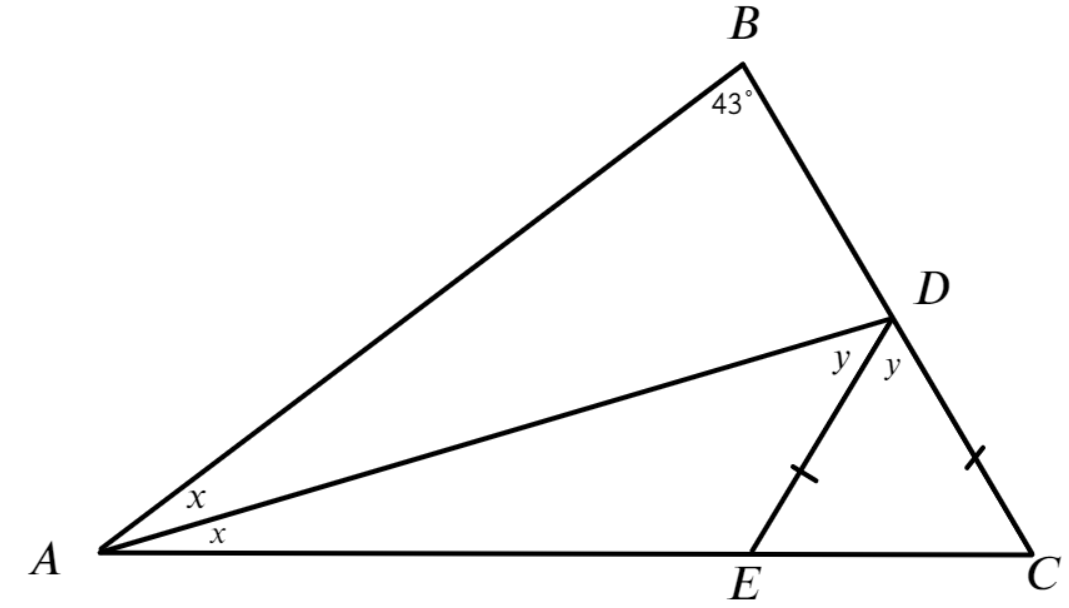
\includegraphics[scale=0.35]{g117.png}}
\end{figure}\\
Обозначим $\angle BAD=\angle DAE=x,\ \angle ADE=\angle EDC=y.$ Тогда $\angle ADB=180^\circ-2y$ и из треугольника $ABD:\ x+43^\circ+180^\circ-2y=180^\circ,\ 2y-x=43^\circ.$ Треугольник $EDC$ является равнобедренным, поэтому $\angle C=(180^\circ-y):2=90^\circ-\frac{1}{2}y.$ Тогда из треугольника $ABC:\ 2x+43^\circ+90^\circ-\frac{1}{2}y=180^\circ,\ 2x-\frac{1}{2}y=47^\circ.$ Домножим второе полученное равенство на 4 и сложим с первым: $2y-x+8x-2y=43^\circ+188^\circ,\ 7x=231^\circ,\ x=33^\circ.$ Значит, $\angle BAC=2\cdot33^\circ=66^\circ.$\newpage\noindent
